\chapter{Evaluation}

 In this chapter, the author investigates the efficiency of the allocation method proposed in the previous chapter, under the distributed quantum computing system with several processors with different number of qubits, different execution time, and the limited network topology.  The following experiments compare the total execution time in each setting among the case of random allocation, the case when only the gate cost is optimized, the case when only the communication cost is optimized, and the case when both costs are optimized.
  
  These experiments were performed by a distributed quantum computing simulator called HeqSim(Heterogeneous Quantum Computing Simulator) [28] that I have developed.
  
\section{Experiment Settings}
 
 Here are the details of the setting of each experiment.
 
\begin{table}[htb]
\centering
  \caption{The details of all experiment settings}
 \begin{tabular}{|c|c|c|c|} \hline
 	\# of Experiment & \# of Processors & \# of total qubits & Network topology \\ \hline
	1 & 2 & 6 & linear \\ \hline
	2 & 4 & 8 & linear \\ \hline
	3 & 4 & 8 & ring \\ \hline
	4 & 4 & 8 & star \\ \hline
	5 & 4 & 8 & random \\ \hline
 \end{tabular}
 \end{table}
 
 \newpage
 
 \section{Experiment 1: Qubit Allocation to Two Quantum Processors}
 
 The first experiment is the simplest one, which is allocation of qubits onto two quantum processors that are connected with each other,  and each processor has different number of qubits and gate execution time.
 
 \begin{figure}[h]
  		\begin{center}
  			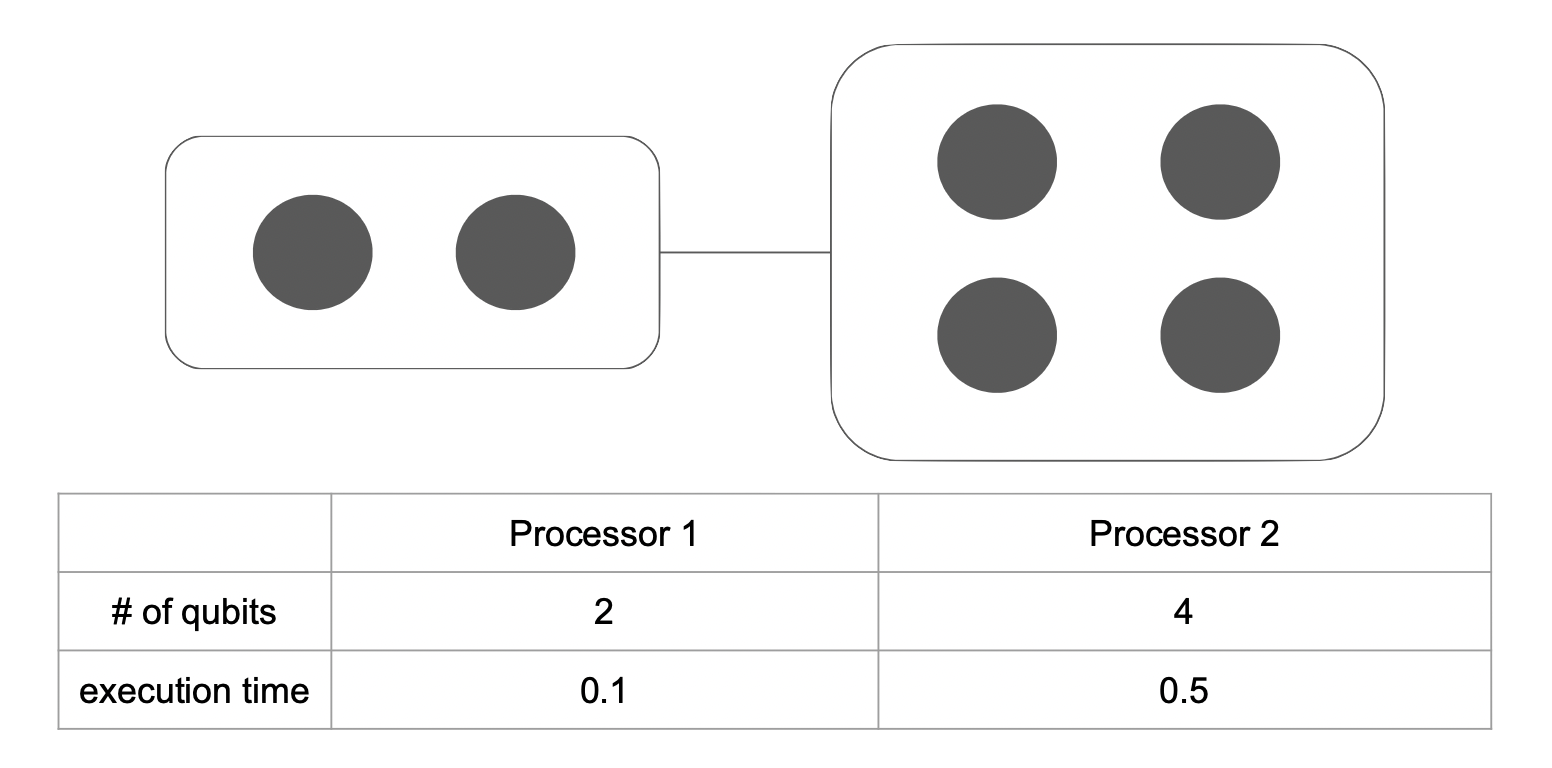
\includegraphics[width=8cm]{img/first_experiment.png}
			\caption{The details of each quantum processor}
			\label{Fig4}
		\end{center}
	\end{figure}
 
 The author executed the following circuit on these two quantum processors.  This circuit is a quantum circuit for solving 6-qubit Simon's problem and also a part of the set of quantum circuits that can be used for benchmarking purpose[20]. 
 \newline
 \newline
 \begin{tikzpicture}
   \begin{yquant}
      qubit {$\ket{\reg_{\idx}}$} q[6];
      
      h q[0];
      h q[1];
      h q[2];
      cnot q[4] | q[2];
      x q[3];
      cnot q[3] | q[2];
      cnot q[3] | q[0, 1];
      x q[0];
      x q[1];
      cnot q[3] | q[0, 1];
      x q[0];
      x q[1];
      x q[3];
      h q[0];
      h q[1];
      h q[2];
   \end{yquant}
\end{tikzpicture}
  \newline
 \newline
 The author compared the total execution time of three different allocation cases, which are when only the gate execution cost is optimized, when only the communication cost is optimized, and when both costs are optimized.  Here is the outcome of this experiment.  (The value in each case is the average value of 10 different execution)
 \newpage
  \begin{figure}[h]
  		\begin{center}
  			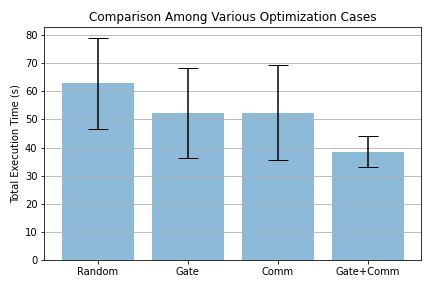
\includegraphics[width=8cm]{img/first_experiment_plot.png}
			\caption{Result of The Experiment1}
			\label{Fig4}
		\end{center}
	\end{figure}
 
 As you can see in the figure above, the case of random allocation was outperformed by the three other cases, and actually the case when gate execution cost was optimized yielded the best result.
 
\section{Experiment 2: Qubit Allocation to Four Quantum Processors (linear topology)}
\section{Experiment 3: Qubit Allocation to Four Quantum Processors (ring topology)}
\section{Experiment 4: Qubit Allocation to Four Quantum Processors (star topology)}
\section{Experiment 5: Qubit Allocation to Four Quantum Processors (random topology)}

%%% Local Variables:
%%% mode: japanese-latex
%%% TeX-master: "../bthesis"
%%% End:
